\section{Task 2}
Conveniently, in task 2 we have the same function and same name for each $v_n$ 
component as we did in Task 1. Therefore, we just need to change the part where 
we introduce errors:
\begin{align*}
    \tilde{v_1} &= \cos(x) (1+\eta_1)\\ 
    \tilde{v_2} &= x^3(1+\eta_2)\\ 
    \tilde{v_3} &= \frac{\tilde{v_1}}{\tilde{v_2}}(1+\eta_3) \\ 
    \tilde{v_4} &= x^2 (1+\eta_4) \\
    \tilde{y} &= (\tilde{v_3} - \tilde{v_4})(1+\eta_5)
\end{align*}
\subsection{Epsilon calculus}
Using the epsilon calculus rules:
\begin{align*}
    \tilde{y} &= \left(
    \frac{\cos(x)}{x^3}\frac{(1+\eta_1)}{(1+\eta_2)}(1+\eta_3) - x^2(1+\eta_4)
    \right) (1+\eta_5) \\
    &= \left(\frac{\cos(x)}{x^3}(1+\eta_1-\eta_2+\eta_3) - x^2(1+\eta_4)\right)(1+\eta_5)\\
    &= y \left(1+ \frac{\cos(x)}{x^3}\frac1y(\eta_1-\eta_2+\eta_3) - x^2\frac1y\eta_4 \right)(1+\eta_5) \\
    &= y \left(1+ \frac{\cos(x)}{x^3}\frac1y(\eta_1-\eta_2+\eta_3) - x^2\frac1y\eta_4 + \eta_5\right) \\
\end{align*}
Finally, we get:
\begin{align*}
K_{A1} &= \displaystyle\frac{
    \left|\frac{\cos(x)}{x^3}\right| + 
    \left|-\frac{\cos(x)}{x^3}\right| +
    \left|\frac{\cos(x)}{x^3}\right| + 
    \left|-x^2\right|}
{\left|\frac{\cos(x)}{x^3} - x^2\right|} + 1\\
\end{align*}

\subsection{Numerical simulation}
In this exercise we simulate the error that we get due to rounding errors.
Here, it is important to note that some errors may interfere such that they add
up, or cancel out. Ideally we would try to calculate each permutation of
$-\eta$ and $+\eta$, as that would yield true max error. However, in practice,
it may take too long to calculate full coverage. Often, we may want to know
just "good enough" approximation of this error. Therefore, we try a number of
randomly selected sample and calculate the error by updating the biggest error.
Exact code solution can be seen in \textit{Description of the numerical methods
and algorithms} section.

\subsection{Comparison of results}
Similarly to results of task 1, both methods do not differ significantly from
one another in terms of results. This can be seen on \ref{fig:task2}, where the
output difference cannot even be seen (due to one point drawn on the other).

\begin{figure}[ht]
    \begin{center}
        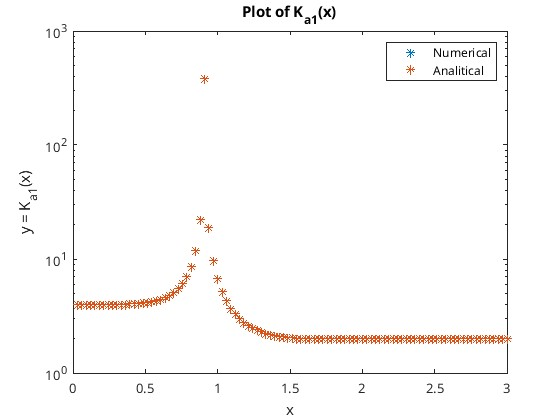
\includegraphics[width=\textwidth]{Task2.jpg}
    \end{center}
    \caption{Comparison of calculating error via numerical and analytical way}
    \label{fig:task2}
\end{figure}
